\documentclass[12pt]{article}

\usepackage[a4paper,left=0.82in,right=0.82in,top=0.9in,bottom=0.95in]{geometry}
\usepackage[T1]{fontenc}
\usepackage[utf8]{inputenc}
\usepackage{lmodern}
\usepackage{amsmath,amssymb,amsthm,mathtools}
\usepackage{booktabs}
\usepackage{array}
\usepackage{microtype}
\usepackage{xcolor}
\usepackage{hyperref}
\usepackage{enumitem}
\usepackage{setspace}

\hypersetup{
  colorlinks=true,
  linkcolor=blue!55!black,
  citecolor=blue!55!black,
  urlcolor=blue!55!black
}

\setstretch{1.055}
\setlength{\parindent}{0pt}
\setlength{\parskip}{0.52em}
\setlist[itemize]{topsep=0.25em,itemsep=0.15em}
\setlist[enumerate]{topsep=0.25em,itemsep=0.15em}

\theoremstyle{plain}
\newtheorem{theorem}{Theorem}
\newtheorem{lemma}[theorem]{Lemma}
\newtheorem{proposition}[theorem]{Proposition}
\newtheorem{corollary}[theorem]{Corollary}
\theoremstyle{definition}
\newtheorem{definition}[theorem]{Definition}
\theoremstyle{remark}
\newtheorem{remark}[theorem]{Remark}

\newcommand{\Lop}{\mathcal L}
\newcommand{\binomtwo}[1]{\binom{#1}{2}}
\newcommand{\floor}[1]{\left\lfloor #1\right\rfloor}
\newcommand{\ceil}[1]{\left\lceil #1\right\rceil}
\newcommand{\supp}{\operatorname{supp}}

\begin{document}

\title{%
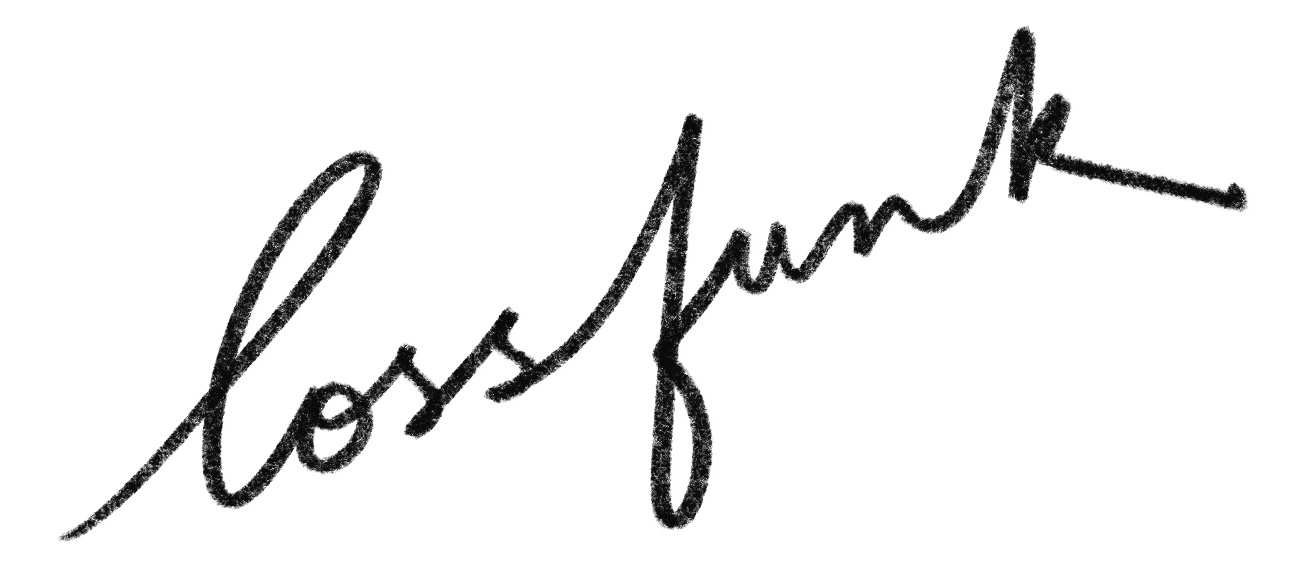
\includegraphics[width=0.33\linewidth]{lossfunk-logo.jpg}\\[0.85cm]
A Colored Turan Proof of the Lollipop Formula}
\author{Siddhartha Mahajan \and Paras Chopra}
\date{\today}
\maketitle

\begin{abstract}
Let \(a_{\Lop}(n)\) be the maximum number of connected regions into which
\(n\) lollipops can divide the plane.  We prove, from Paulsen's two geometric
obstructions, the exact four-cluster formula
\[
  a_{\Lop}(n)=4\binom n2+S(n)+n+1,
\]
where
\[
  \begin{aligned}
  S(n)=
  \max_{a+b+c+d=n,\;0\le a\le b\le c\le d}\;
  &\left(3\sum_{1\le i<j\le4}m_i m_j-2ab\right),\\
  &(m_1,m_2,m_3,m_4)=(a,b,c,d).
  \end{aligned}
\]
The proof is entirely combinatorial after the geometric reduction.  It uses a
colored Zykov symmetrization, a weighted blocker lemma, and an exact
\(3\times4\) matrix inequality.  The matrix inequality is proved by support
compression: alternating four-edge path compressions and double-star
compressions reduce every integer matrix to star-forest normal form, where the
efficient degree pattern is \(K_{1,2}\cup K_2\cup K_2\).  This also explains
the asymptotic cluster proportions
\[
  \frac{3}{16},\frac{3}{16},\frac{5}{16},\frac{5}{16}.
\]
\end{abstract}

\section{The formula}

A \emph{lollipop} is a circle together with a half-line attached at one point
of the circle and extending radially outward.  We assume arrangements are
generic: there are no tangencies, no triple intersection points, and no
intersection occurs at an anchor point.  This entails no loss for a maximum,
since a non-generic arrangement can be perturbed without decreasing the number
of regions.

Let \(C\) be the total number of crossings between distinct lollipops.  Adding
one generic lollipop with \(k\) crossings increases the number of regions by
\(k+1\), and hence
\begin{equation}\label{eq:regions}
  \#\hbox{regions}=C+n+1.
\end{equation}
Thus the problem is to maximize \(C\).

For \(n\ge0\), define
\begin{equation}\label{eq:Sdef}
  S(n)=\max_{a+b+c+d=n,\;0\le a\le b\le c\le d}
  \left(3\sum_{1\le i<j\le4}m_i m_j-2ab\right),
  \qquad (m_1,m_2,m_3,m_4)=(a,b,c,d).
\end{equation}
Equivalently, for a fixed multiset of four cluster sizes, the penalized pair is
the pair with smallest product, i.e. the two smallest clusters.

\begin{theorem}\label{thm:lollipop-formula}
For every \(n\ge0\),
\begin{equation}\label{eq:main-formula}
  a_{\Lop}(n)=4\binom n2+S(n)+n+1.
\end{equation}
\end{theorem}

The first values obtained from \eqref{eq:main-formula} are
\[
\begin{gathered}
1,2,10,25,45,71,104,142,186,237,294,356,425,500,580,667,\\
761,859,964,1076,1193,1316,1446,1581,1722,1870,2024,2183,\\
2349,2521,2698,2882,3073.
\end{gathered}
\]

\section{Geometric input and the two-graph reduction}

We use Paulsen's terminology.  A pair of lollipops is \emph{close} if the
angle between the two stem directions is at most \(90^\circ\).  A pair is
\emph{intriguing} if the two circles either do not meet, or meet at angle at
most \(90^\circ\), after orienting the two circles in the same direction.

The following geometric facts are due to Cutler--Karlsson--Sloane and Paulsen.
The present paper is a self-contained proof of the combinatorial extremal step
that follows from these facts.

\begin{lemma}[geometric lollipop input]\label{lem:geometry}
For a generic pair of lollipops:
\begin{enumerate}[label=(\roman*)]
  \item any pair has at most \(7\) crossings;
  \item a close pair has at most \(5\) crossings;
  \item an intriguing pair has at most \(5\) crossings;
  \item a pair that is both close and intriguing has at most \(4\) crossings.
\end{enumerate}
Furthermore, among any four lollipops there is a close pair, and among any five
lollipops there is an intriguing pair.
\end{lemma}

\begin{remark}
In the Lean formalization the geometric input is not treated as a single
undifferentiated assumption.  The strongest current upper boundary asks for
distinct circle and ray-supporting-line facts for each unordered pair; from
these facts Lean now constructs the finite carrier-intersection witness and
the automatic crossing table for the generic \(7\)-crossing branch.  The
remaining upper inputs are named Euclidean route certificates which imply the
component-wise \(5\)- and \(4\)-crossing savings for the close, intriguing, and
close-and-intriguing branches.  These routes include disjoint or nested
circles, projection-distance or determinant/Cauchy separation of mixed
circle-ray components, half-line outward separation when a ray starts outside a
circle and points away from its center, and parallel-offset separation of
ray-ray components.
The close-direction interface is also split: Lean proves the trigonometric
bridge from cyclic normalized closeness to a nonnegative dot product of
bearing vectors, and records a normalized-bearing compatibility condition
which turns this into a statement about the actual stored ray vectors.
Since close radial pairs need not make one mixed circle-ray component empty,
the Lean geometry folder also records a direct whole-carrier savings interface
for coupled component-count proofs.  Two direct coupled overlap theorems are
now formalized: if two overlap witnesses together improve all four component
estimates, then the whole carrier intersection has at most five points; if one
point lies in all four components, then the whole carrier intersection has at
most four points, under the standard noncoincident-circle and
noncoincident-ray-line hypotheses.  Lean also proves that a point lying in any
three of the four lifted circle/ray product components automatically lies in
the fourth component, so a triple-overlap witness gives the stronger
four-point bound; likewise, a two-double-overlap certificate whose two
witnesses coincide is converted to the same four-component bound.  Lean uses
the four-component form to turn
the shared-anchor close-route audit example into an actual \(4\)-crossing
direct carrier-savings certificate.
Lean converts the routes to component-savings bounds and assembles the
automatic pair certificates into the upper input used by the colored-Turan
proof.  It also has a direct-savings automatic boundary whose close and
intriguing inputs are whole-carrier cardinality certificates, so the coupled
overlap theorems can feed the final Theorem~\ref{thm:lollipop-formula}
boundary without first being decomposed into four independent component
caps.  The theorem-facing subtheorem index now also exposes the route
transport lemmas explicitly: named \(5\)- and \(4\)-crossing routes convert to
component-savings certificates, direct carrier-savings certificates, and the
corresponding local or global rational pair-crossing bounds.  The separate Lean modules
\path{CompleteFormalization/FiniteCarrier.lean} and
\path{CompleteFormalization/AutomaticUpper.lean} contain this reduction, and
\path{CompleteFormalization/Proof.lean} indexes the resulting theorem
boundary and proves Theorem~\ref{thm:lollipop-formula} from it.  A separate
\path{EndToEndFormalization/} folder also exports theorem endpoints whose
lower input is finite carrier-subset data for the produced blow-ups, so the
upper and lower automatic-carrier reductions can be combined without changing
the older proof stack; its \path{Statement.lean} and \path{Subtheorems.lean}
files record the statement, the named proved bridge lemmas, and the most
concrete current certificate boundary in one place.  In that boundary,
triple-overlap, two-double-overlap, and all-four-overlap certificates are
converted by Lean into the direct whole-carrier savings needed for the
close/intriguing branches, with triple-overlap exposed as a direct
\(4\)-crossing savings route and coincident two-double overlap exposed the
same way.  The lower side can also be stated using
cardinality lower bounds on the automatic carrier finsets themselves; when
such a bound is supplied, Lean uses the automatic finset as the local lower
witness.  The current theorem-facing statement uses Lean's canonical
sorted-quad cluster witness internally, so this boundary no longer exposes a
separate cluster-map witness as an input.  The
all-four-overlap interface also has a common-anchor constructor: if two
primitive lollipops share their anchor point, Lean proves that point lies in
all four lifted circle/ray components and hence supplies the direct
\(4\)-crossing savings certificate under the usual noncoincidence hypotheses.
The same interface now has a primitive-point constructor: any coordinate
point certified to lie on both primitive circles and both primitive rays
produces the all-four and five-overlap witnesses, and hence the corresponding
direct \(4\)- and \(5\)-crossing savings certificates under the same
noncoincidence hypotheses.  It also has a primitive triple-overlap constructor:
ordinary coordinate membership facts showing that one point lies in any three
of the four circle/ray product components are converted to all-four overlap,
primitive five-overlap, and direct \(4\)- and \(5\)-crossing savings
certificates.  The two-double-overlap interface now has primitive coordinate
constructors as well: Lean accepts ordinary circle/ray membership facts for
two coordinate points in each of the three component-pair patterns, builds the
lifted two-double witness, and derives the direct \(5\)-crossing savings
certificate.  When the two-double witnesses are the same primitive coordinate
point, Lean also derives the all-four overlap witness and the direct
\(4\)-crossing savings certificate.  These \(4\)-crossing primitive witnesses
are bundled in a flexible primitive four-overlap boundary, so the
close-and-intriguing branch may use all-four, triple, or same-point two-double
coordinate data before converting to the existing primitive upper certificate.
Lean exposes this flexible primitive upper boundary with the canonical
automatic-cardinality lower boundary, and with the component-indexed,
table-exact,
finset-exact, component-covered, component-finset, disjoint component-finset,
and indexed disjoint component-finset lower endpoints.
The clean statement/proof index also re-exports the exact indexed-carrier,
finite-carrier, common-anchor lower, automatic-cardinality, and canonical
Karlsson lower-table bridge lemmas, re-exports the route/direct-savings/overlap
upper transport lemmas, and exposes the common-anchor and raw primitive
all-four/five direct-savings aliases at the theorem-facing layer.  Its split
boundary now also has overlap, primitive, and flexible primitive
component-indexed and indexed-disjoint-component endpoints, where the lower
construction supplies disjoint component point families, with or without exact
component-carrier coverage.
At the stepwise family level, Lean also
has a primitive
overlap upper certificate whose close/intriguing fields are these raw
coordinate overlap witnesses rather than prebuilt lifted component-overlap
objects.  This primitive upper certificate converts to the existing automatic
overlap boundary, and the theorem-facing endpoint combines it with exact
indexed carrier enumerations plus one equality to the canonical Karlsson
lower table.
Direct carrier-savings certificates are also monotone in their bound in Lean,
so a stronger certificate, such as a \(4\)-crossing saving, can be reused
wherever the upper proof only asks for a \(5\)-crossing saving.
The
Euclidean derivation of the route certificates for a concrete lollipop model
remains part of the model-specific geometric work.
\end{remark}

Given an arrangement of \(n\) lollipops, define graphs \(D,E\) on the same
vertex set by
\[
  ij\in D\quad\Longleftrightarrow\quad L_i,L_j\hbox{ are not close},
\]
\[
  ij\in E\quad\Longleftrightarrow\quad L_i,L_j\hbox{ are not intriguing}.
\]
By Lemma \ref{lem:geometry},
\begin{equation}\label{eq:forbidden-DE}
  D\hbox{ is }K_4\hbox{-free},\qquad E\hbox{ is }K_5\hbox{-free}.
\end{equation}
For a pair \(ij\), Lemma \ref{lem:geometry} gives the pointwise estimate
\begin{equation}\label{eq:pair-weight}
  c_{ij}\le
  4+\mathbf 1_{ij\in D}+\mathbf 1_{ij\in E}+\mathbf 1_{ij\in D\cap E}.
\end{equation}
Therefore
\begin{equation}\label{eq:two-graph-bound}
  C\le 4\binom n2+\sigma(D,E),
  \qquad
  \sigma(D,E):=|D|+|E|+|D\cap E|.
\end{equation}
Theorem \ref{thm:lollipop-formula} is now reduced to the following colored
Turan theorem.

\begin{theorem}[colored Turan theorem]\label{thm:colored-turan}
If \(D\) is \(K_4\)-free and \(E\) is \(K_5\)-free on the same \(n\)-vertex
set, then
\begin{equation}\label{eq:sigma-upper}
  \sigma(D,E)\le S(n).
\end{equation}
\end{theorem}

The proof occupies Sections \ref{sec:zykov}--\ref{sec:matrix}.  The lower
construction is given in Section \ref{sec:lower}; together with
\eqref{eq:regions} and \eqref{eq:two-graph-bound}, it proves Theorem
\ref{thm:lollipop-formula}.

\section{Colored Zykov symmetrization}\label{sec:zykov}

Color every unordered pair of vertices with one of four colors:
\[
  0: \hbox{neither }D\hbox{ nor }E,
  \qquad
  A: E\hbox{-only},
\]
\[
  B: D\hbox{-only},
  \qquad
  X: D\cap E.
\]
These colors have weights
\[
  w(0)=0,\\quad w(A)=1,
  \quad w(B)=1,
  \quad w(X)=3,
\]
so that \(\sigma(D,E)\) is the total color-weight.

\begin{lemma}[colored Zykov reduction]\label{lem:zykov}
An extremal pair \((D,E)\) for \(\sigma\) may be chosen as a blow-up of a
complete colored quotient: the vertex set is partitioned into classes
\(V_1,\ldots,V_k\), every pair inside one class has color \(0\), and every pair
between two distinct classes has one fixed color from \(\{A,B,X\}\).  In
particular, there are no color-\(0\) pairs between distinct classes.
\end{lemma}

\begin{proof}
Suppose \(uv\) has color \(0\).  Let \(d_w(v)\) be the total color-weight from
\(v\) to all vertices other than \(u,v\).  If \(d_w(u)\le d_w(v)\), replace
\(u\) by a clone of \(v\): for every \(z\ne u,v\), give \(uz\) the same color
as \(vz\), while keeping \(uv\) color \(0\).  This operation changes \(\sigma\)
by \(d_w(v)-d_w(u)\ge0\).

It cannot create a \(K_4\) in \(D\).  Indeed, a new \(D\)-clique using the
clone \(u\) and not \(v\) corresponds to the same clique with \(v\) in place of
\(u\), while a clique using both \(u\) and \(v\) is impossible because \(uv\) is
not a \(D\)-edge.  The same argument forbids creation of a \(K_5\) in \(E\).
Thus the operation preserves \eqref{eq:forbidden-DE} and does not decrease
\(\sigma\).

More explicitly, among all pairs satisfying \eqref{eq:forbidden-DE} and
maximizing \(\sigma\), choose one that maximizes the ordered twin-pair
potential
\[
  \Phi=\sum_v |\{z:\hbox{ the color-row of }z\hbox{ equals the color-row of }v\}|.
\]
For a color-\(0\) pair \(uv\), maximality of \(\sigma\) forces
\(d_w(u)=d_w(v)\), since cloning in either direction is allowed.  Hence either
clone keeps \(\sigma\) maximal.  If \(u\) and \(v\) are not already twins, clone
the vertex with the smaller twin class to the one with the larger twin class.
This strictly increases \(\Phi\): the cloned vertex joins the larger twin
class, while every other twin class loses at most the cloned vertex.  This
contradicts the choice of the tie-breaker.  Therefore every color-\(0\) pair is
a twin pair.  Consequently color-\(0\) is an equivalence relation, its classes
are twin classes, and between two distinct classes all pairs have one fixed
nonzero color.  This is the claimed quotient form.
\end{proof}

Let the quotient class sizes be \(x_1,\ldots,x_k\), with
\(\sum_i x_i=n\), and put
\[
  Q=\sum_i x_i^2.
\]
Let
\[
  a=\sum_{ij\in A}x_i x_j,
  \qquad
  b=\sum_{ij\in B}x_i x_j,
\]
where \(A\) and \(B\) now also denote the graphs of \(A\)-colored and
\(B\)-colored quotient edges.  The total cross-class mass is
\[
  P=\sum_{i<j}x_i x_j=\frac{n^2-Q}{2}.
\]
Since \(X\)-edges have weight \(3\), while \(A\)- and \(B\)-edges have weight
\(1\),
\begin{equation}\label{eq:sigma-quotient}
  \sigma=3P-2a-2b=\frac32(n^2-Q)-2a-2b.
\end{equation}

The forbidden cliques translate into blocker conditions.  Since
\(D\) consists of colors \(B\cup X\), every four quotient vertices contain an
\(A\)-edge; otherwise they form a \(K_4\) in \(D\).  Thus
\begin{equation}\label{eq:alphaA}
  \alpha(A)\le3.
\end{equation}
Similarly, since \(E\) consists of colors \(A\cup X\),
\begin{equation}\label{eq:alphaB}
  \alpha(B)\le4.
\end{equation}

\section{The weighted blocker lemma}\label{sec:blocker}

For nonnegative integer weights \(x_1,\ldots,x_k\) with total \(n\), define
\(Q=\sum_i x_i^2\).  If \(G\) is a graph on \([k]\), write
\[
  w(G)=\sum_{ij\in E(G)}x_i x_j.
\]

For \(r\ge1\), let
\[
  \rho_r(x)=\min_{\mathcal P}\sum_{P\in\mathcal P}
  \left(\sum_{i\in P}x_i\right)^2,
\]
where the minimum is over all partitions of \([k]\) into \(r\) possibly empty
parts.

\begin{lemma}[weighted Turan theorem]\label{lem:weighted-turan}
If \(G\) is \(K_{r+1}\)-free, then
\begin{equation}\label{eq:weighted-turan}
  w(G)\le\frac12\bigl(n^2-\rho_r(x)\bigr).
\end{equation}
\end{lemma}

\begin{proof}
The usual Zykov symmetrization works with vertex weights: if two nonadjacent
vertices have different weighted neighborhoods, clone the smaller weighted
neighborhood to the larger one.  This preserves \(K_{r+1}\)-freeness and does
not decrease \(w(G)\).  In an extremal graph, two nonadjacent vertices of
positive weight must therefore have the same weighted neighborhood.  It follows
that nonadjacency is transitive on the positive-weight vertices: otherwise two
nonadjacent positive vertices would have different adjacency to a third
positive vertex.  Hence the induced graph on the positive-weight support is
complete multipartite.  Since \(G\) is \(K_{r+1}\)-free, this positive-weight
multipartite graph has at most \(r\) parts; vertices of weight zero may be
assigned to the parts arbitrarily.  For a partition with part weights
\(s_1,\ldots,s_r\), its edge weight is
\[
  \sum_{i<j}s_i s_j=\frac12\left(n^2-\sum_i s_i^2\right),
\]
which is maximized exactly when \(\sum_i s_i^2\) is minimized.
\end{proof}

Define
\begin{equation}\label{eq:Mdef}
  M(n)=\min_{a+b+c+d=n,\;a,b,c,d\in\mathbb Z_{\ge0}}
  \left[\frac32(a^2+b^2+c^2+d^2)+2ab\right].
\end{equation}
Since
\[
  \frac32n^2-
  \left[\frac32(a^2+b^2+c^2+d^2)+2ab\right]
  =3\sum_{i<j}m_i m_j-2ab,
\]
where \((m_1,m_2,m_3,m_4)=(a,b,c,d)\), and since the two variables in the
penalized product may be labelled as the two smallest cluster sizes, the
definitions imply
\begin{equation}\label{eq:S-M}
  S(n)=\frac32 n^2-M(n).
\end{equation}

\begin{lemma}[weighted blocker lemma]\label{lem:blocker}
Let \(A,B\) be graphs on \([k]\) with \(\alpha(A)\le3\) and
\(\alpha(B)\le4\).  With the notation above,
\begin{equation}\label{eq:blocker}
  \frac32Q+2w(A)+2w(B)\ge M(n).
\end{equation}
\end{lemma}

\begin{proof}
The complement of \(A\) is \(K_4\)-free.  By Lemma \ref{lem:weighted-turan},
\[
  \frac12(n^2-Q)-w(A)
  \le \frac12(n^2-\rho_3(x)),
\]
and hence
\begin{equation}\label{eq:a-lower}
  w(A)\ge\frac12(\rho_3(x)-Q).
\end{equation}
Likewise, the complement of \(B\) is \(K_5\)-free, so
\begin{equation}\label{eq:b-lower}
  w(B)\ge\frac12(\rho_4(x)-Q).
\end{equation}
Combining \eqref{eq:a-lower} and \eqref{eq:b-lower},
\begin{equation}\label{eq:rho-bound}
  \frac32Q+2w(A)+2w(B)
  \ge \rho_3(x)+\rho_4(x)-\frac12Q.
\end{equation}

Choose partitions attaining \(\rho_3(x)\) and \(\rho_4(x)\), and intersect
them.  This gives a \(3\times4\) nonnegative integer matrix
\(U=(u_{ij})\), where \(u_{ij}\) is the total weight lying in the \(i\)-th
part of the \(3\)-partition and the \(j\)-th part of the \(4\)-partition.
Let
\[
  r_i=\sum_j u_{ij},\qquad c_j=\sum_i u_{ij}.
\]
Then
\[
  \rho_3(x)=\sum_i r_i^2,
  \qquad
  \rho_4(x)=\sum_j c_j^2.
\]
Also
\[
  Q=\sum_\ell x_\ell^2\le \sum_{i,j}u_{ij}^2,
\]
because squaring after grouping can only increase the sum of squares.  Thus
\eqref{eq:rho-bound} gives
\[
  \frac32Q+2w(A)+2w(B)
  \ge
  \sum_i r_i^2+
  \sum_j c_j^2-\frac12\sum_{i,j}u_{ij}^2.
\]
The right side is at least \(M(n)\) by the matrix theorem proved in
Section \ref{sec:matrix}.
\end{proof}

We now prove Theorem \ref{thm:colored-turan}, assuming the matrix theorem for a
moment.

\begin{proof}[Proof of Theorem \ref{thm:colored-turan}]
By Lemma \ref{lem:zykov}, assume \((D,E)\) is in quotient form.  Then
\eqref{eq:alphaA} and \eqref{eq:alphaB} allow Lemma \ref{lem:blocker}, so
\[
  \frac32Q+2a+2b\ge M(n).
\]
Using \eqref{eq:sigma-quotient},
\[
  \sigma
  =\frac32n^2-\left(\frac32Q+2a+2b\right)
  \le \frac32n^2-M(n)=S(n),
\]
by \eqref{eq:S-M}.  This proves \eqref{eq:sigma-upper}.
\end{proof}

\section{The \texorpdfstring{\(3\times4\)}{3 x 4} matrix theorem}\label{sec:matrix}

For a \(3\times4\) nonnegative integer matrix \(U=(u_{ij})\) with total sum
\(n\), row sums \(r_i\), and column sums \(c_j\), put
\begin{equation}\label{eq:Fdef}
  F(U)=\sum_{i=1}^3 r_i^2+
        \sum_{j=1}^4 c_j^2-\frac12\sum_{i,j}u_{ij}^2.
\end{equation}

\begin{theorem}[matrix theorem]\label{thm:matrix}
For every \(3\times4\) nonnegative integer matrix \(U\) of total sum \(n\),
\begin{equation}\label{eq:matrix-theorem}
  F(U)\ge M(n).
\end{equation}
\end{theorem}

The proof is the main technical point.  Think of the positive entries of
\(U\) as edge masses on the bipartite graph \(K_{3,4}\), whose left vertices
are the rows and whose right vertices are the columns.  If two positive cells
share a row or a column, call the corresponding edges adjacent.  Expanding
\eqref{eq:Fdef} gives
\begin{equation}\label{eq:F-edge}
  F(U)=\frac32\sum_e u_e^2+2\sum_{e\sim f}u_eu_f.
\end{equation}
Here the second sum is over unordered pairs of distinct adjacent support
edges.

\subsection*{Compression to a star forest}

The next lemma is the normal-form step needed below: every matrix can be
compressed to a star forest without increasing \(F\).  Equality may occur during
compression, so the conclusion concerns the compressed matrix rather than the
original support.

\begin{lemma}[support compression]\label{lem:compression}
For every nonnegative integer matrix \(U\), there is a nonnegative integer
matrix \(U'\) with the same total sum such that
\[
  F(U')\le F(U)
\]
and the support graph of \(U'\) is a forest whose connected components are
stars.
\end{lemma}

\begin{proof}
We repeatedly apply a support-decreasing move.  Since the support has at most
twelve edges, it is enough to show that every non-star support admits one such
move preserving the total mass and not increasing \(F\).  In each alternating
move below, \(\varepsilon\) is restricted to the integer interval on which all
changed entries remain nonnegative.  This interval contains \(0\), and its two
endpoints are obtained by killing at least one entry on one of the two
alternating classes.  Hence endpoint moves keep the matrix integral, do not
create new support edges, and strictly decrease the support unless the matrix
was already outside the case under discussion.

The graph-theoretic bookkeeping used here is finite.  In \(K_{3,4}\), every
non-star support, after relabeling rows and columns, falls into one of the
following descent shapes: a four-cycle, a four-edge path in one of the two
orientations, or a diameter-\(3\) double-star with its remaining leaves in the
corresponding double-star envelope.  The Lean formalization proves this
classification by exhaustive checking over the twelve possible support edges;
the paragraphs below prove the descent move for each canonical shape.

First suppose the support contains a cycle.  Since the support graph is
bipartite, the cycle is even.  Add \(\varepsilon\) and \(-\varepsilon\)
alternately around the cycle.  Row sums and column sums, and therefore the
first two terms of \eqref{eq:Fdef}, remain fixed.  The final term
\(-\frac12\sum u_{ij}^2\) is a concave quadratic in \(\varepsilon\).  The
allowed integer interval is obtained by requiring the entries on the
decreasing half of the cycle to stay nonnegative in each direction.  One
endpoint of this interval does not increase \(F\): if both endpoints had larger
value than at \(0\), concavity would force the value at \(0\) to be larger than
itself by interpolation between the endpoints.  The chosen endpoint makes at
least one formerly positive entry zero and creates no new positive entries,
because every edge being changed already lies in the support.

Thus we may next assume that the support is a forest.  If a tree component has
diameter at least \(4\), choose four consecutive edges on a path in that
component, with masses \(x_1,x_2,x_3,x_4\).  Replace them by
\[
  x_1+\varepsilon,
  \quad x_2-\varepsilon,
  \quad x_3+\varepsilon,
  \quad x_4-\varepsilon.
\]
The total mass is preserved.  The three internal vertex sums on this four-edge
path are unchanged; only the two endpoint vertex sums change.  In the expression
\eqref{eq:F-edge}, the coefficient of \(\varepsilon^2\) is
\[
  2-\frac12\cdot4=0,
\]
so \(F\) is linear in \(\varepsilon\) on the allowed integer interval.  One
endpoint of that interval does not increase \(F\) according to the sign of this
linear function, and kills at least one of the four entries, again without
creating a new support edge.

It remains to treat a forest component of diameter exactly \(3\), i.e. a
double-star.  This is the only remaining non-star case: a forest with no path
of four edges and no component of diameter \(3\) has every component of
diameter at most \(2\), hence is a star forest.
Let \(y\) be the mass of the central edge.  Choose a leaf edge of mass \(x\)
on one side and a leaf edge of mass \(z\) on the other.  Let \(A\) be the sum
of the other leaf-edge masses incident with the center on the \(x\)-side, and
let \(B\) be the analogous sum on the \(z\)-side.  If we delete the central
edge and add its mass \(y\) to the \(x\)-edge, a direct calculation from
\eqref{eq:F-edge} gives the change
\[
  F_{\rm old}-F_x = y(2B+2z-x).
\]
If instead we add \(y\) to the \(z\)-edge, then
\[
  F_{\rm old}-F_z = y(2A+2x-z).
\]
At least one of these two quantities is nonnegative: otherwise
\(x>2B+2z\ge2z\) and \(z>2A+2x\ge2x\), impossible.  Hence one of the two
operations preserves the total mass, keeps all masses integral and
nonnegative, deletes the central edge, and does not increase \(F\).  Repeating
this step removes all diameter-\(3\) components.

Each move strictly decreases the number of positive entries, and the support
cardinality is a nonnegative integer.  Therefore the process terminates, and
when it terminates no cycle, no four-edge path in a tree, and no double-star
component remains.  A forest component with no path of four edges and no
diameter-\(3\) double-star has diameter at most \(2\), so it is a star.  The
final support is therefore a star forest, proving the lemma.
\end{proof}

\subsection*{Star forests}

For a star component with \(t\) positive edges of masses
\(z_1,\ldots,z_t\) and total mass \(s=\sum_\ell z_\ell\), its contribution to
\(F\) is
\begin{equation}\label{eq:star-cost}
  s^2+\frac12\sum_{\ell=1}^t z_\ell^2.
\end{equation}
In particular,
\begin{equation}\label{eq:star-efficiency}
  s^2+\frac12\sum_{\ell=1}^t z_\ell^2
  \ge \left(1+\frac1{2t}\right)s^2
  =\frac{s^2}{\eta_t},
  \qquad
  \eta_t:=\frac{2t}{2t+1}.
\end{equation}

\begin{lemma}[star-forest minimum]\label{lem:star-forest}
If \(U\) is a nonnegative integer matrix whose support is a star forest, then
\(F(U)\ge M(n)\), where \(n\) is the total sum of its entries.
\end{lemma}

\begin{proof}
If \(n=0\), then \(F(U)=M(0)=0\).  Hence assume \(n>0\).  Let the star
components have degrees \(t_\nu\) and total masses \(s_\nu\).  If the degree
list is not \((2,1,1)\), then
\begin{equation}\label{eq:Gamma-bound}
  \Gamma:=\sum_\nu \eta_{t_\nu}\le2.
\end{equation}
Indeed, one or two components give \(\Gamma<2\), since each \(\eta_t<1\).  If
there are three components, then the seven vertices of \(K_{3,4}\) allow only
\((2,1,1)\) or \((1,1,1)\); excluding \((2,1,1)\) leaves \((1,1,1)\), for
which \(\Gamma=3\cdot(2/3)=2\).  Here a star with \(t\) positive edges uses
\(t+1\) support vertices.  Thus three nonempty components with largest degree
at least \(3\), or with two components of degree at least \(2\), would require
at least eight support vertices, impossible in \(K_{3,4}\).  There cannot be
four nonempty star components, because each such component contains at least
one row vertex and the components are disjoint while there are only three
rows.

By \eqref{eq:star-efficiency} and Cauchy's inequality,
\[
  F(U)\ge\sum_\nu\frac{s_\nu^2}{\eta_{t_\nu}}
  \ge\frac{(\sum_\nu s_\nu)^2}{\sum_\nu\eta_{t_\nu}}
  =\frac{n^2}{\Gamma}
  \ge\frac{n^2}{2}.
\]
For \(n\ge4\), the balanced quadruple in \eqref{eq:Mdef} gives
\(M(n)\le n^2/2\).  Explicitly, for \(n=4q+r\), use
\((q,q,q,q)\), \((q,q,q,q+1)\), \((q,q,q+1,q+1)\), or
\((q,q+1,q+1,q+1)\) according as \(r=0,1,2,3\).  The resulting value is at
most \(n^2/2\) for \(n\ge4\).  For \(n\le3\), the identity
\[
  F(U)=\frac32n
      +3\sum_{i,j}\binom{u_{ij}}2
      +2\sum_{\substack{(i,j)<(i',j')\\
             (i=i'\;\text{or}\;j=j'),\;(i,j)\ne(i',j')}}u_{ij}u_{i'j'}
\]
shows \(F(U)\ge\frac32n=M(n)\).  Thus every non-\((2,1,1)\) star forest
satisfies the desired bound.

Now suppose the degree list is \((2,1,1)\).  The degree-two star must be
centered at a row vertex: if it were centered at a column vertex, only one row
vertex would remain for the two disjoint \(K_2\) components.  Thus, up to row
and column permutation, its four positive edge masses are
\[
  \begin{pmatrix}
  a&b&0&0\\
  0&0&c&0\\
  0&0&0&d
  \end{pmatrix}.
\]
For this matrix,
\[
  F(U)=(a+b)^2+c^2+d^2+\frac12(a^2+b^2+c^2+d^2)
  =\frac32(a^2+b^2+c^2+d^2)+2ab.
\]
Since \(a+b+c+d=n\), this is at least \(M(n)\) by definition.
\end{proof}

\begin{proof}[Proof of Theorem \ref{thm:matrix}]
Apply Lemma \ref{lem:compression} to replace \(U\) by a star-forest matrix
\(U'\) with the same total sum and \(F(U')\le F(U)\).  Lemma
\ref{lem:star-forest} gives \(F(U')\ge M(n)\).  Hence \(F(U)\ge M(n)\).
\end{proof}

The Lean formalization follows this proof split at the level of checked
subtheorems: the proved support-descent theorem and the proved star-forest
minimum theorem give the proved matrix theorem.  The support-descent proof uses
the finite relabeling/exhaustion described above, and the star-forest proof is
checked by exhausting the canonical star-forest support cases.  More
precisely, Lean proves the finite star-forest shape classification, the
non-star descent classification, the one-step descent theorem, the canonical
case package, the star-forest minimum, and the final matrix theorem under the
names
\begin{center}
\begin{tabular}{@{}l@{}}
\texttt{isSupportStarForest\_iff\_canonicalShape},\\
\texttt{nonstar\_support\_has\_descent\_shape},\\
\texttt{support\_descent\_step\_proven},\\
\texttt{canonicalStarForestMinimumCases\_proven},\\
\texttt{starForestMinimum\_proven},\\
\texttt{matrix\_theorem\_proven}.
\end{tabular}
\end{center}
The separate theorem-facing assembly files import these proved Section 5
endpoints into the displayed Theorem 1 statement.  Thus the matrix theorem is
not a remaining Lean input to Theorem \ref{thm:colored-turan}.

\section{The lower construction}\label{sec:lower}

The lower construction uses Karlsson's optimal four-lollipop configuration
from \cite{CKS}.  We use only the following crossing table for that base
configuration.  Label the four base lollipops so that their pairwise crossing
table is
\[
\begin{array}{c|cccc}
 &1&2&3&4\\
\hline
1&*&5&7&7\\
2&&*&7&7\\
3&&&*&7\\
4&&&&*
\end{array}
\]
Thus the pair \((1,2)\) contributes \(5\) crossings and the other five pairs
contribute \(7\) crossings.

\begin{lemma}[blow-up stability]\label{lem:blowup}
Assume the four-lollipop base configuration with the crossing table displayed
above.
For any nonnegative integers \(m_1,m_2,m_3,m_4\), there is a generic
arrangement of \(m_1+m_2+m_3+m_4\) lollipops whose crossing number is
\begin{equation}\label{eq:lower-L}
  L(m_1,m_2,m_3,m_4)
  =4\sum_i\binom{m_i}{2}
   +5m_1m_2
   +7\sum_{\substack{i<j\\(i,j)\ne(1,2)}}m_i m_j.
\end{equation}
\end{lemma}

\begin{proof}
Replace the \(i\)-th base lollipop by \(m_i\) sufficiently small, mutually
generic perturbations.  Transverse crossings between two distinct base
lollipops persist under sufficiently small perturbation in the bounded
circle--circle and mixed circle--ray components.  For the unbounded ray
components this is not a compactness consequence by itself: small changes of
ray directions can create intersections far from the base configuration.  The
perturbation must therefore be chosen with explicit coordinate inequalities
certifying the full primitive carrier intersection for every affected pair
(equivalently, with the local finite-carrier certificates used in the Lean
boundary).  Under those local certificates, every pair from two different
clusters has the same crossing number as the corresponding base pair.

Inside one cluster, choose the copies in a tiny one-parameter family obtained
by small translations and small independent rotations of the stem direction.
For two sufficiently close copies of one lollipop, the two circles meet in two
points, each stem meets the other circle once, and the two stems do not meet;
these four intersections are transverse and persist under a generic small
perturbation.  Therefore every intra-cluster pair contributes exactly \(4\)
crossings.  A final arbitrarily small perturbation removes accidental triple
points without changing any pairwise crossing count.
\end{proof}

\begin{remark}
In the Lean formalization this lower construction is represented by the
theorem-facing certificate package
\[
  {\small\texttt{KarlssonBaseBlowUpIncrementalLowerData}}
\]
and, more locally, by
\[
  {\small\texttt{KarlssonBaseSixPairBlowUpIncrementalLowerData}},
\]
where the base table is supplied as the six displayed unordered entries plus
symmetry.  The checked part expands that six-entry table to the universal
base-pair table and can also assemble the copy-pair crossing values from one
local certificate for each blown-up pair.  It then converts the construction
to the pairwise lower interface, sums the inherited cluster table, and derives
the ordered-insertion region equation.  The current Lean boundary also has a
stepwise form in which each insertion step is supplied locally and Lean
assembles the recurrence; for the exact OEIS four-base table, the displayed
\(1\to2\to8\to23\to45\) region arithmetic is recorded in this stepwise form.
The complete Lean index also exports the six-entry base-table certificate, the
unordered base sum \(40\), the resulting base region count \(45\), and the
canonical four-fiber cluster witness used in the finite pair-counting collapse.
For the exceptional exact OEIS pair \((Q_0,Q_1)\), Lean also checks the
cyclic-close fact, Paulsen's strict obtuse-intersection condition showing the
pair is not intriguing, and a half-line-outward route proving the local
\(\le 5\) crossing and finite-witness-cardinality bounds from the six-pair
base-coordinate certificate.  Lean also proves that all four exact OEIS base
qoppas have normalized-bearing compatibility, so the recorded normalized
directions agree with the actual coordinate ray vectors.  The separate
complete-formalization OEIS
geometry file now also names an explicit ray-ray intersection point and proves
that the mixed component \(\mathrm{ray}(Q_0)\cap\mathrm{circle}(Q_1)\) consists
only of the two x-axis points with coordinates \((9\pm\sqrt{57})/20\), forcing
any exact six-pair finite witness to contain at least those two points.  It
also solves the circle-circle component: the exact radical-axis
relation \(20045x+40y=3\) and the two radical-coordinate circle-circle
witnesses are proved in Lean, and together with the ray-ray and ray-circle
points they give a five-point finset whose coercion is exactly the primitive
\((Q_0,Q_1)\) carrier intersection.  Thus Lean now constructs the local
\((Q_0,Q_1)\) coordinate crossing certificate directly.  For every
non-exceptional exact base pair
\((Q_0,Q_2)\), \((Q_0,Q_3)\), \((Q_1,Q_2)\), \((Q_1,Q_3)\), and
\((Q_2,Q_3)\), the complete Lean folder also constructs all seven component
points, proves their carrier memberships and distinctness, derives automatic
finite-witness cardinality \(7\), and exports the local coordinate crossing
certificates.  The end-to-end Lean folder now packages these six exact
automatic carrier-cardinality facts as the Nat-valued OEIS base lower table:
the exceptional base pair contributes \(5\), and the five non-exceptional base
pairs contribute \(7\).  Lean also relabels the exact OEIS base arrangement by
the canonical all-ones cluster witness and proves the same automatic lower
table in those canonical labels.  In this relabeled base case, Lean also uses
the automatic carrier finset itself as the local lower subset and constructs
the local monotone lower certificate consumed by the pairwise lower interface.
The Euclidean realization of the local blow-ups with exactly these pairwise
crossing values remains a model-specific geometric certificate, not a hidden
algebraic assumption.  In particular, the unbounded ray cases in
Lemma~\ref{lem:blowup} require concrete coordinate or local perturbation
certificates; they do not follow from a bare compactness argument.  Lean now
also includes a monotone pairwise lower
interface:
\[
  {\small\texttt{PairwiseCardinalityClusteredKarlssonBlowUpIncrementalLowerBoundData}},
\]
where a concrete construction only has to prove that each blown-up pair has at
least the corresponding Karlsson table value.  Lean sums these pairwise
inequalities over unordered pairs and derives a lower-bound attainment
statement from the ordered region recurrence.  The local geometric bridge is
also formalized in
\path{PrimitiveGeometry/LowerWitness.lean}: a finite set of distinct points
inside one carrier intersection, together with the ordinary local
carrier-crossing certificate for the full pair intersection, gives the
required local monotone copy-pair lower certificate.  The new
\texttt{IndexedLowerWitness} file turns an
injective indexed family of \(k\) explicit carrier points into a \(k\)-point
lower subset and hence, with a local carrier certificate, into a
\(\texttt{pairCross}\ge k\) lower bound.  The companion
\texttt{IndexedCarrier} file handles the exact-enumeration form: if an
injective indexed family has image equal to the whole primitive carrier
intersection, Lean converts it into the local or pairwise finite-carrier
crossing certificate, computes the corresponding automatic finite-carrier
cardinality and automatic crossing-table entry, and also recovers the
corresponding lower subset.  Lean also proves that this exact image equality
can be supplied by showing indexed-point membership plus coverage of all
carrier points, or by covering the four primitive component cases
circle-circle, circle-ray, ray-circle, and ray-ray separately.  The
\texttt{AutomaticCardinalityWitness} file pushes
the same indexed point data directly to the automatic carrier finset
cardinality inequality used by the strongest lower boundary.  The
theorem-facing statement also exposes an
\(\texttt{IndexedPointCertificate}\) endpoint: with overlap-witness upper data,
explicit indexed lower point families of the canonical \(4\), \(5\), and \(7\)
sizes imply Theorem~\ref{thm:lollipop-formula}.  Its
\(\texttt{ComponentIndexedPointCertificate}\) variant is a lower-bound-only
component version: four disjoint component point families are enumerated as
one canonical lower-point family, without requiring the construction to prove
that those points cover the whole carrier intersection.  Its
\(\texttt{ExactIndexedCarrierCertificate}\) variant strengthens the lower
input to exact indexed enumerations of the whole canonical primitive pair
carriers and derives the indexed-point boundary internally.  The
\(\texttt{TableExactIndexedCarrierCertificate}\) variant reduces the
remaining pair-table bookkeeping to one equality with the canonical rational
Karlsson lower table, from which Lean derives the increasing-entry and
non-increasing-entry facts.  A finset-exact carrier variant lets the
construction supply each exact finite carrier set directly, together with
its set equality and cardinality, instead of manufacturing an indexed
enumeration.  Lean also proves that this finite-set equality can be derived
from finite-set membership plus carrier coverage, or from separate coverage
of the four circle/ray component cases; these helpers identify the supplied
finite set with the automatic carrier finset and compute the corresponding
automatic cardinality and crossing-table entry.  The theorem-facing Lean
layer now also exposes this component-covered finite-carrier form as a full
endpoint: the construction supplies the finite set, membership, the four
component-coverage fields, and the cardinality, while Lean derives exactness
internally.  A still more component-local endpoint lets the construction
supply four finite sets, one for each of the circle-circle, circle-ray,
ray-circle, and ray-ray components; Lean unions those sets and derives the
same component-covered carrier boundary.  A disjoint component-finset
endpoint now also derives that union cardinality from pairwise disjointness,
four component cardinalities, and a single component-size sum.  An indexed
disjoint component-finset endpoint goes one step closer to coordinate
verification by taking each component set to be the image of an injective
indexed point family, but this exact endpoint still includes component
coverage of the whole carrier.  The new
\texttt{LowerAnchorWitness} file proves the
basic shared-anchor case of this bridge: a common anchor is an actual
primitive carrier-intersection point, giving a one-point lower subset and,
with a local carrier certificate, a \(\texttt{pairCross}\ge1\) bound.  This
does not by itself supply the required \(4\), \(5\), or \(7\) lower
multiplicities.  The separate
\texttt{AutomaticLower} module composes this with
the automatic finite-carrier table: if the produced pair table agrees with
the automatic table and the construction supplies these lower subsets, Lean
assembles the monotone lower certificate used by
Theorem~\ref{thm:lollipop-formula}.  It also contains a specialized
Nat-valued form of the Karlsson lower table, where the construction supplies
subsets of sizes \(4\), \(5\), or \(7\) directly and Lean proves that this
natural-number table coerces to the rational cluster table.  A further
automatic-cardinality form lets the construction prove that the automatic
carrier finset itself has the required cardinality lower bound; Lean then uses
that finset as the lower witness.  The strongest current statement builds in
Lean's canonical sorted-quad cluster witness, leaving only the canonical
carrier-cardinality inequalities to be supplied on the lower side.  The OEIS
four-base case of those automatic cardinality inequalities is already proved
from the exact five- and seven-point certificates, including the canonical
all-ones relabeling used by the theorem-facing lower boundary and its local
monotone lower certificates.  Lean now also proves the matching upper table
for this canonical all-ones base case: the concrete \((Q_0,Q_1)\)
half-line-outward route gives a direct whole-carrier \(\le 5\) certificate in
both orientations, and the close/non-intriguing classification of this
exceptional pair is lifted through the canonical relabeling to prove that its
canonical case bound is exactly \(5\).  The generic noncoincident carrier
theorem gives \(\le 7\) for the other canonical base pairs.  Lean also proves,
from exact normalized directions, that all five non-exceptional OEIS base pairs
are not close, and from strict Paulsen obtuse-distance inequalities that every
distinct exact OEIS base pair is non-intriguing.  These facts lift through the
canonical all-ones relabeling, so every non-exceptional canonical pair has case
bound exactly \(7\), and the canonical automatic pair table satisfies the
canonical case bound for every base pair.  These upper inequalities combine
with the lower table to give exact equality between the canonical automatic
pair table and the rational Karlsson cluster table.  Lean also sums this exact
automatic table to \(40\) and proves the corresponding base-region arithmetic
\(45=\mathrm{pairSum}+4+1\).  The new
\path{TheoremOneAssembly/} folder presents the theorem-facing Lean endpoint in
statement/subtheorems/proof order, and
\path{StatementProof/EndpointTheorems.lean} re-exports the proved
complete-formalization theorem endpoints under the clean statement/proof
namespace.  Thus future concrete blow-up geometry need not classify every
extra intersection away in order to prove the lower-bound half.
\end{remark}

Subtracting \(4\binom n2\) from \eqref{eq:lower-L}, with
\(n=m_1+m_2+m_3+m_4\), gives
\[
  L(m_1,m_2,m_3,m_4)-4\binom n2
  =3\sum_{i<j}m_i m_j-2m_1m_2.
\]
For a fixed multiset of four cluster sizes, the product penalized by the
coefficient \(-2\) should be the smallest product.  Hence the best blow-up has
\[
  \max L(m_1,m_2,m_3,m_4)=4\binom n2+S(n).
\]
By \eqref{eq:regions}, this gives
\begin{equation}\label{eq:lower-bound}
  a_{\Lop}(n)\ge4\binom n2+S(n)+n+1.
\end{equation}

The upper bound follows from Lemma \ref{lem:geometry}, Theorem
\ref{thm:colored-turan}, and \eqref{eq:two-graph-bound}.  Thus
\eqref{eq:lower-bound} is sharp, proving Theorem \ref{thm:lollipop-formula}.

\section{Numerical table and asymptotics}

The continuous relaxation of \eqref{eq:Mdef} is minimized at
\[
  a=b=\frac{3n}{16},\qquad c=d=\frac{5n}{16}.
\]
Consequently
\[
  S(n)=\frac{33}{32}n^2+O(1),
\]
and
\[
  a_{\Lop}(n)=4\binom n2+\frac{33}{32}n^2+n+O(1)
  =\frac{97}{32}n^2-n+O(1).
\]

\begin{table}[htbp]
\centering
\begin{tabular}{@{}c c r r@{}}
\toprule
\(n\)&one optimal \((a,b,c,d)\)&\(S(n)\)&\(a_{\Lop}(n)\)\\
\midrule
0&(0,0,0,0)&0&1\\
1&(0,0,0,1)&0&2\\
2&(0,0,1,1)&3&10\\
3&(0,1,1,1)&9&25\\
4&(1,1,1,1)&16&45\\
5&(1,1,1,2)&25&71\\
6&(1,1,2,2)&37&104\\
7&(1,2,2,2)&50&142\\
8&(1,2,2,3)&65&186\\
9&(1,2,3,3)&83&237\\
10&(2,2,3,3)&103&294\\
11&(2,2,3,4)&124&356\\
12&(2,2,4,4)&148&425\\
13&(2,3,4,4)&174&500\\
14&(2,3,4,5)&201&580\\
15&(2,3,5,5)&231&667\\
16&(3,3,5,5)&264&761\\
17&(3,3,5,6)&297&859\\
18&(3,3,6,6)&333&964\\
19&(3,4,6,6)&372&1076\\
20&(4,4,6,6)&412&1193\\
21&(4,4,6,7)&454&1316\\
22&(4,4,7,7)&499&1446\\
23&(4,5,7,7)&545&1581\\
24&(4,5,7,8)&593&1722\\
25&(4,5,8,8)&644&1870\\
26&(5,5,8,8)&697&2024\\
27&(5,5,8,9)&751&2183\\
28&(5,5,9,9)&808&2349\\
29&(5,6,9,9)&867&2521\\
30&(5,6,9,10)&927&2698\\
\bottomrule
\end{tabular}
\caption{Values from the closed formula.}
\end{table}
\section*{Acknowledgments}

We thank David O. H. Cutler, Jonas Karlsson, Neil J. A. Sloane, and Matthias
Paulsen for the lollipop problem and for the geometric ideas on which this
note builds.  OpenAI's ChatGPT was used during exploratory algebra checking,
finite-case audit organization, and drafting assistance.
\begin{thebibliography}{9}

\bibitem{CKS}
David O. H. Cutler, Jonas Karlsson, and Neil J. A. Sloane,
\emph{Cutting a Pancake with an Exotic Knife},
arXiv:2511.15864v3 [math.CO], 19 Apr. 2026.
\url{https://arxiv.org/abs/2511.15864}.

\bibitem{Paulsen}
Matthias Paulsen,
\emph{The Lollipop Problem}, 2026.
\url{https://math.mp42.de/lollipop/}.

\bibitem{OEIS}
OEIS Foundation Inc.,
\emph{The On-Line Encyclopedia of Integer Sequences}, entry A389624,
``Maximum number of regions that can be formed in the plane by drawing
\(n\) lollipop (or qoppa) shapes of any size and orientation.''
\url{https://oeis.org/A389624}.

\bibitem{Turan}
P. Turan,
On an extremal problem in graph theory,
\emph{Matematikai es Fizikai Lapok} \textbf{48} (1941), 436--452.

\bibitem{Zykov}
A. A. Zykov,
On some properties of linear complexes,
\emph{Matematicheskii Sbornik} \textbf{24} (1949), 163--188.

\end{thebibliography}

\clearpage
\appendix

\section{Paulsen's forced intriguing pair}\label{app:paulsen}

We recall the short linear-algebra proof that among five circles some pair is
intriguing.  Suppose five circles with centers \(x_i\in\mathbb R^2\) and radii
\(r_i>0\) are pairwise non-intriguing.  Then every pair intersects at an
obtuse angle, equivalently
\begin{equation}\label{eq:obtuse}
  r_i^2+r_j^2<|x_i-x_j|^2<(r_i+r_j)^2.
\end{equation}
For each circle set
\[
  v_i=\frac1{r_i}(1,\,r_i^2-|x_i|^2,\,x_i)\in\mathbb R^4,
\]
and endow \(\mathbb R^4\), written as triples \((\alpha,\beta,x)\), with the
symmetric bilinear form
\[
  \langle(\alpha,\beta,x),(\alpha',\beta',x')\rangle
  =\frac12\alpha\beta'+\frac12\beta\alpha'+x\cdot x'.
\]
A direct calculation using \eqref{eq:obtuse} gives
\[
  \langle v_i,v_i\rangle=1,
  \qquad
  -1<\langle v_i,v_j\rangle<0\quad(i\ne j).
\]
Five vectors in \(\mathbb R^4\) are linearly dependent.  Move the negative
terms in a nontrivial relation to the other side.  Both sides are nonempty:
the first coordinate of every \(v_i\) is \(1/r_i>0\), so a nontrivial linear
relation cannot have all coefficients with the same sign.  Thus
\[
  \sum_{i\in P}a_i v_i=\sum_{j\in N}b_j v_j,
  \qquad a_i,b_j>0,
\]
with \(P,N\) nonempty and disjoint.  Replacing the relation by its negative if
necessary, assume \(|P|\le2\).  Put \(w=\sum_{i\in P}v_i\).  If \(|P|=1\),
then \(\langle\sum_{i\in P}a_i v_i,w\rangle>0\).  If
\(P=\{1,2\}\), it equals
\((a_1+a_2)(1+\langle v_1,v_2\rangle)>0\).  But
\[
  \left\langle\sum_{j\in N}b_j v_j,w\right\rangle<0,
\]
since all cross inner products are negative.  This contradicts the linear
relation.  Therefore five pairwise non-intriguing circles cannot exist.

\end{document}
